\documentclass[12pt]{beamer}

\hypersetup{colorlinks=true,linkcolor = blue}
\usetheme{Warsaw}

\usepackage[utf8]{inputenc}
\usepackage[russian,english]{babel}
\usepackage[T2A]{fontenc}

\usepackage{hyperref}
\usepackage[final]{listings}
\usepackage{breakurl}
\usepackage{cite}
\usepackage{perpage}

\def\Url\Breaks{\do\/\do-}

\lstset{
  frame=single,
  breaklines=true,
  basicstyle=\small,
  postbreak=\raisebox{0ex}{\ensuremath{\hookrightarrow\space}},
  numbers=left
}

\MakePerPage{footnote}

\title{Operating Systems}
\subtitle{Memory Allocation}
\author{Me}
\date{\today}

\begin{document}

  \begin{frame}
    \titlepage
  \end{frame}

  \begin{frame}
\frametitle{План лекции}
\begin{itemize}
  \item Назначение распределенных файловых систем.
  \item Взаимодействие клиента и сервера. Andrew File System.
  \item Распределение метаданных ФС.
  \item Консенсус и связанные задачи.
  \item Ненадежный канал связи. Задача двух генералов.
  \item Асинхронные системы. FLP Impossibility. Paxos.
\end{itemize}
\end{frame}

  \section{Карта памяти}

Получение карты памяти - это чисто формальная часть задания. На самом деле
карта памяти предоставляется multiboot загрузчиком. Те кто не использует
предоставленный bootstrap.S должны будут разобраться с получением карты памяти
самостоятельно. Для всех остальных эта инструкция.

\subsection{Получение карты памяти}

Собственно, bootstrap.S уже получает \emph{физический} адрес multiboot
information structure, формат которого приведен в~\cite{multiboot} (раздел 3.3
Boot information format), вам остается только проверить, что поля mmap\_length и
mmap\_addr валидны\footnote{Для этого разберитесь с описанием поля flags} и
распарсить и использовать эту информацию.

Чтобы получить адрес multiboot information structure добавьте в свой код
следующие строки:

\begin{lstlisting}
extern const uint32_t mboot_info;
\end{lstlisting}

После этого вы можете использовать mboot\_info - в этой переменной и содержится
адрес multiboot information structure. Обратите внимание, на тип - uint32\_t:
\begin{itemize}
  \item вам нужно подключить заголовок stdint.h, чтобы использовать этот тип;
  \item адерс 32-битный, т. е. находится в первых 4GB физической памяти.
\end{itemize}

Несмотря на то, что адрес multiboot information structure физический мы можем
преобразовать его к указателю, так как у нас есть настроенный identity mapping
в начальной таблице страниц, который покрывает первые 4GB памяти.

\subsection{Резервирование памяти ядра}

Карта памяти получается (условно) от аппаратуры компьютера, которая ничего не
знает о ядре ОС. Соответственно, в этой карте памяти не отображено, что часть
памяти занята ядром ОС - вам необходимо зарезервировать эту память
самостоятельно. В противном случае ваши аллокаторы могут ее аллоцировать и вы
перезапишите уже занятую память.

Для того чтобы этого не случилось вам нужно получить границы памяти занятой
ядром ОС, для этого добавьте в код следующие строки:

\begin{lstlisting}
extern char text_phys_begin[];
extern char bss_phys_end[];
\end{lstlisting}

После чего вы можете преобразовать text\_phys\_begin в 64 битное число\footnote{
На самом деле старшие 32 бита должны быть нулевыми.} которое содержит физический
адрес начала вашего ядра, а если вы преобразуете bss\_phys\_end в число, то
получите адрес конца ядра.

  \begin{frame}
\frametitle{Примитивная задача планирования}

Cписок задач (даже пока не потоков) дан заранее:
\begin{itemize}
  \item<2-> про каждую задачу известна ее длительность;
  \item<3-> задача работает от начала и до конца (не прерываясь, не вытесняясь);
  \item<4-> какой смысл вообще что-то придумывать в такой ситуации?
\end{itemize}
\end{frame}

\begin{frame}
\frametitle{Пример}

\begin{columns}[T]
  \begin{column}{.4\textwidth}
    \begin{figure}
      \centering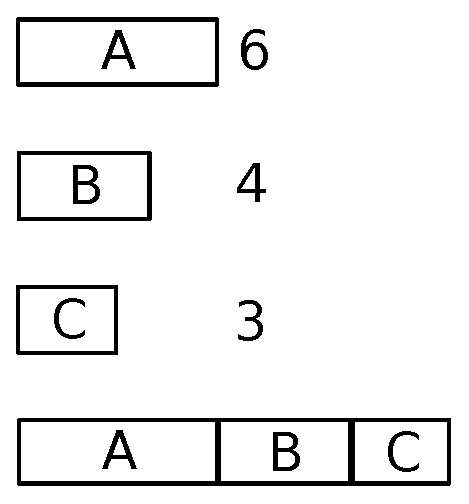
\includegraphics[width=.9\linewidth]{sched0}
      \caption{Example Schedule}
    \end{figure}
  \end{column}
  \begin{column}{.6\textwidth}
    \begin{itemize}
      \item<2-> $TOTAL = 6 + 4 + 3 = 13$
      \item<3-> $WAIT_A = 6$
      \item<3-> $WAIT_B = 6 + 4 = 10$
      \item<3-> $WAIT_C = 6 + 4 + 3 = 13$
      \item<4-> $WAIT_{AVG} = {\left(6 + 10 + 13\right)\over 3} = 9.\left(6\right)$
    \end{itemize}
  \end{column}
\end{columns}
\end{frame}

\begin{frame}
\frametitle{Пример}

\begin{columns}[T]
  \begin{column}{.4\textwidth}
    \begin{figure}
      \centering\includegraphics[width=.9\linewidth]{sched1}
      \caption{Example Schedule}
    \end{figure}
  \end{column}
  \begin{column}{.6\textwidth}
    \begin{itemize}
      \item<2-> $TOTAL = 6 + 4 + 3 = 13$
      \item<3-> $WAIT_C = 3$
      \item<3-> $WAIT_B = 3 + 4 = 7$
      \item<3-> $WAIT_A = 6 + 4 + 3 = 13$
      \item<4-> $WAIT_{AVG} = {\left(3 + 7 + 13\right)\over 3} = 7.\left(6\right)$
    \end{itemize}
  \end{column}
\end{columns}
\end{frame}

\begin{frame}
\frametitle{Shortes Job First}

Shortest Job First (SJF) - гарантирует минимальное \emph{среднее} время ожидания завершения задачи.

\onslide<2>{\emph{Доказательство:} ну это же очевидно!}
\end{frame}

\begin{frame}
\frametitle{Shortes Job First}

\emph{Доказательство:}
\begin{itemize}
  \item планируем $N$ задач, с временами работы $T_0$, $T_1$, ..., $T_{N-1}$;
  \item допустим, что в расписании с наименьшим $WAIT_{AVG}$ есть две
        задачи $s$ и $t$, такие что $T_s > T_t$, но $s$ идет раньше чем $t$;
  \item поменяем местами $s$ и $t$ в расписании;
  \item все задачи до $t$ и начиная с $s$ имеют тоже самое время ожидания;
  \item все задачи начиная с $t$ и до $s$ имеют меньшее время ожидания;
  \item получили раписание с меньшим $WAIT_{AVG}$ - противоречие.
\end{itemize}
\end{frame}

\begin{frame}
\frametitle{Ввод и вывод}

\begin{itemize}
  \item<1-> задачи могут обращаться к медленным внешним устройствам или ждать
            внешних событий:
              \begin{itemize}
                \item задача, которая только ждет - бесполезно занимает
                      процессор (естественная точка перепланирования);
              \end{itemize}
  \item<2-> задачу стоит снять с процессора:
     \begin{itemize}
       \item если задача не критична к времени отклика, то стоит использовать
             прерывания;
       \item если внешнее устройство обрабатывает запросы долго, то стоит
             использовать прерывания;
       \item если время ожидания не предсказуемо (получение пакета по сети или
             ожидание нажатия клавиши), то стоит использовать прерывания;
     \end{itemize}
\end{itemize}
\end{frame}

\begin{frame}
\frametitle{Пример}

\begin{columns}[T]
  \begin{column}{.4\textwidth}
    \begin{figure}
      \centering\includegraphics[width=1.0\linewidth]{iosched0}
      \caption{Schdeule with IO}
    \end{figure}
  \end{column}
  \begin{column}{.6\textwidth}
    \begin{itemize}
      \item в расписании могут появляться "дыры" (все ждут завершения IO)
      \item интуиция - хотим, максимально параллельный IO:
        \begin{itemize}
          \item реалистично для сети или клавиатуры;
          \item не реалистично, например, для диска - общий ресурс.
        \end{itemize}
    \end{itemize}
  \end{column}
\end{columns}
\end{frame}

\begin{frame}
\frametitle{Пример}

\begin{columns}[T]
  \begin{column}{.4\textwidth}
    \begin{figure}
      \centering\includegraphics[width=1.0\linewidth]{iosched1}
      \caption{Schdeule with IO}
    \end{figure}
  \end{column}
  \begin{column}{.6\textwidth}
    \begin{itemize}
      \item задачу с ближайшим IO пропускаем вперед:
        \begin{itemize}
          \item чем раньше задача начнет IO, тем лучше;
          \item чем больше задач будет выполнять IO параллельно, тем лучше;
          \item при прочих равных, задачу с большим IO стоит пустить раньше;
          \item получаем SJF с учетом IO;
        \end{itemize}
    \end{itemize}
  \end{column}
\end{columns}
\end{frame}

\begin{frame}
\frametitle{Ограничения}

\begin{itemize}
  \item<1-> мы не знаем заранее время до следующего IO (или завершения)
        \begin{itemize}
          \item мы можем его примерно оценить основывась на "истории" работы
                задачи;
        \end{itemize}
  \item<2-> список задач не дан заранее
        \begin{itemize}
          \item SJF теряет свою оптимальность в этом случае (трудно планировать
                без полной информации и без возможности изменить решение);
          \item для оптимального планирования нам нужно вытеснять задачи в
                произвольные моменты времени (вытесняющая многозадачность);
        \end{itemize}
  \item<3-> IO зависит от внешних условий (пользователь, нагрузка, другие
            задачи);
\end{itemize}
\end{frame}

\begin{frame}
\frametitle{Round Robin}

Сделаем ограничения более реалистичными (переходим от задач к потокам):
\begin{itemize}
  \item<1-> мы можем снимать поток с процессора в любое время (не спрашивая
        разрешения у потока):
        \begin{itemize}
          \item когда задача запускает операцию ввода/вывода;
          \item по сигналу от таймера;
        \end{itemize}
  \item<2-> больше мы ничего не знаем о потоке.
\end{itemize}
\end{frame}

\begin{frame}
\frametitle{Round Robin}

Если мы ничего не знаем о потоках - дадим каждому по чуть-чуть по очереди:
\begin{itemize}
  \item<2-> нужно ограничить время работы на процессоре (квант времени)
        \begin{itemize}
          \item поток может "заблокироваться" раньше, чем истечет квант времени;
        \end{itemize}
  \item<3-> все активные потоки выполняются по очереди
        \begin{itemize}
          \item если поток отработал квант, ставим его в конец очереди;
          \item если поток "разблокировался", ставим его в конец очереди;
        \end{itemize}
  \item<4-> Round Robin дает гарантии реального времени:
        \begin{itemize}
          \item зная, сколько всего потоков мы можем посчитать максимальное
                время ожидания;
        \end{itemize}
\end{itemize}
\end{frame}

\begin{frame}
\frametitle{Что не так с Round Robin?}

Рассмотрим планирование нескольких задач из двух классов:
\begin{enumerate}
  \item<2-> CPU bounded - не блокируются, постоянно вырабатывают свой квант:
        \begin{itemize}
          \item например, какие-то численные расчеты попадают в этот класс;
        \end{itemize}
  \item<3-> IO bounded - работают мало, ждут долго - не вырабаывтают свой квант:
        \begin{itemize}
          \item например, текстовый редактор большую часть времени ждет ввода;
        \end{itemize}
\end{enumerate}
\end{frame}

\begin{frame}
\frametitle{Что не так с Round Robin?}
\begin{figure}
  \only<1>{\centering\includegraphics[width=.6\linewidth]{rr0}}
  \only<2>{\centering\includegraphics[width=.6\linewidth]{rr1}}
  \only<3>{\centering\includegraphics[width=.6\linewidth]{rr2}}
  \only<4>{\centering\includegraphics[width=.6\linewidth]{rr3}}
  \only<5>{\centering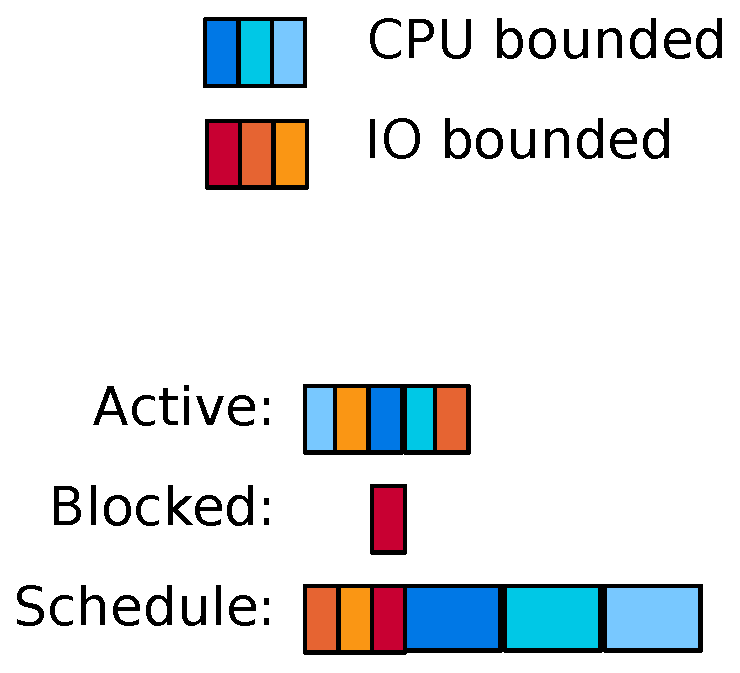
\includegraphics[width=.7\linewidth]{rr4}}
  \only<6>{\centering\includegraphics[width=.7\linewidth]{rr5}}
  \only<7>{\centering\includegraphics[width=.8\linewidth]{rr6}}
  \only<8>{\centering\includegraphics[width=.9\linewidth]{rr7}}
  \caption{Round Robin Example}
\end{figure}
\end{frame}

\begin{frame}
\frametitle{Что не так с Round Robin?}

\begin{itemize}
  \item<1-> IO bounded потоки получают много меньше CPU, а ждут столько же:
    \begin{itemize}
      \item это кажется не честным;
      \item IO bounded потоки - это, часто, интерактивные потоки (т. е.
            пользователь не доволен);
    \end{itemize}
  \item<2-> нужна возможность учитывать разные классы задач:
    \begin{itemize}
      \item в примере мы могли ставить IO bounded задачи в начало (осторожно,
            может приводить к старвации!);
      \item приоритетизация задач:
            \begin{itemize}
              \item IO bounded vs CPU bounded;
              \item внутри класса можно варьировать квант времени;
            \end{itemize}
    \end{itemize}
\end{itemize}
\end{frame}

  \begin{frame}
\frametitle{Продвинутые алгоритмы аллокации памяти}
\framesubtitle{Аллокация в несколько этапов}

Современные аллокаторы памяти выделяют две стадии:

\begin{itemize}
  \item<2-> аллокация больших блоков (Buddy Allocator и Ко.):
    \begin{itemize}
      \item аллокации просиходят нечасто, большие объекты живут долго
      \item чем больше блок тем меньше накладные расходы на служебные структуры алокатора - можем хранить больше информации
    \end{itemize}
  \item<3-> аллокация маленьких блоков фиксированного размера (SLAB и Ко.):
    \begin{itemize}
      \item блоки фиксированного размера проще аллоцировать
      \item блоки фиксированного размера требуют меньше служебной информации
      \item блоки имеют одинаковый размер не случайно - часто это объекты одного типа и это можно использовать
    \end{itemize}
\end{itemize}

\end{frame}

\begin{frame}
\frametitle{Buddy Allocator}
\framesubtitle{Вводные положения}

\begin{itemize}
  \item вся аллоцируемая память разбита на большие блоки фиксированного размера (будем называть их PAGE)
  \item каждому PAGE поставлен в соответсвие дескриптор (мы легко можем получить дескриптор по номеру PAGE и наоборот, считайте, что у нас есть массив таких дескрипторов), хранящий служебную информацию (свободен/занят, порядок свободного блока)
  \item память аллоцируется и освобождается блоками по $2^i\times PAGE$, $i$ будем называть порядком блока
  \item порядок блока хранит пользователь и передает его в как функцию аллокации, так и в функцию освобождения
\end{itemize}
\end{frame}

\begin{frame}
\frametitle{Buddy Allocator}
\framesubtitle{Buddies}

Ключевой концепцией для Buddy Allocator-а является понятие Buddy:
\begin{itemize}
  \item Buddy Allocator хранит информацию о блоках в отдельных списках по порядкам этих блоков (т. е. для каждого возможного порядка блока есть свой список);
  \item cмежные (в памяти, а не в списке) блоки одного пордяка называются Buddies (plural for buddy);
  \item два смежных блока (Buddies) в обединении дают один блок большего порядка, и наоборот из одного блока можно полуить два Buddies меньшего порядка.
\end{itemize}

\end{frame}

\begin{frame}
\frametitle{Buddy Allocator}
\framesubtitle{Buddyies}

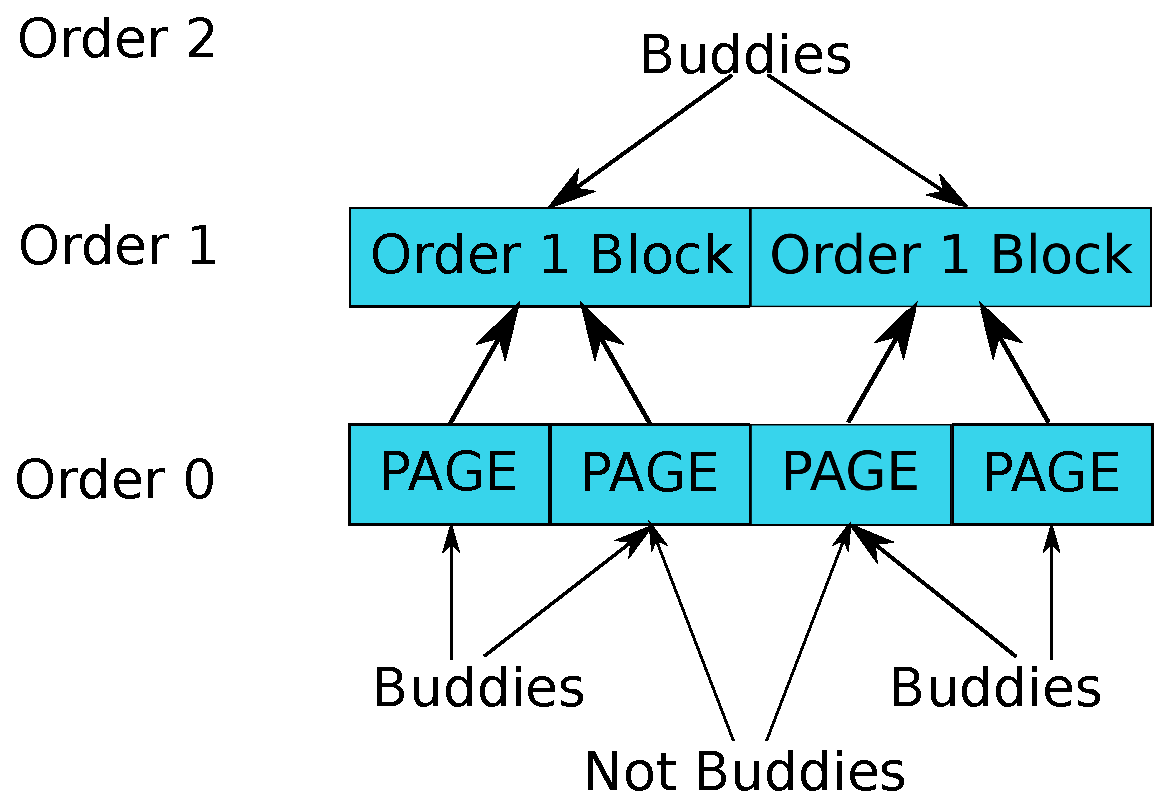
\includegraphics[width=.9\linewidth]{buddy-buddies}

\end{frame}

  \begin{frame}
\frametitle{SLAB Allocator}
\framesubtitle{Аллокация маленьких объектов фиксированного размера}

Теперь решаем еще более простую задачу - аллокацию "маленьких" объектов фиксированного размера:
\begin{itemize}
  \item мы умеем аллоцировать большие блоки - будем использовать их как пулы;
  \item аллоцируем блоки фиксированного размера из пула - тривиально;
  \item объекты одного размера уменьшают вероятность фрагментации;
  \item как на этом построить универсальный аллокатор (malloc/free)?
\end{itemize}

\end{frame}

\begin{frame}
\frametitle{SLAB Allocator}

Базовым понятием для SLAB аллокатора является (неожиданно) SLAB:
\begin{itemize}
  \item SLAB - это пулл объектов одинакового размера;
  \item аллокатор может иметь в распоряжении несколько SLAB-ов - при необходимости аллоцируются новые SLAB-ы;
  \item каждому объекту в SLAB-е соответствует дескриптор (по сути, нужен, чтобы связать объекты в список);
\end{itemize}
\end{frame}

\begin{frame}
\frametitle{SLAB Allocator}
\framesubtitle{Разделение на большие и маленькие объекты}

SLAB аллокатор делит объекты далее на большие и маленькие, и использует для них разную структуру SLAB-ов:
\begin{itemize}
  \item разделение нужно чтобы уменьшить потери памяти для больших объектов;
  \item нет четкой границы, что считать большим объектом, а что маленьким;
  \item обычно маленькими объектами считают объекты меньше $1/8$ размера PAGE (минимального размера пула).
\end{itemize}

\end{frame}

\begin{frame}
\frametitle{SLAB Allocator}
\framesubtitle{Организация SLAB-а маленьких объектов}

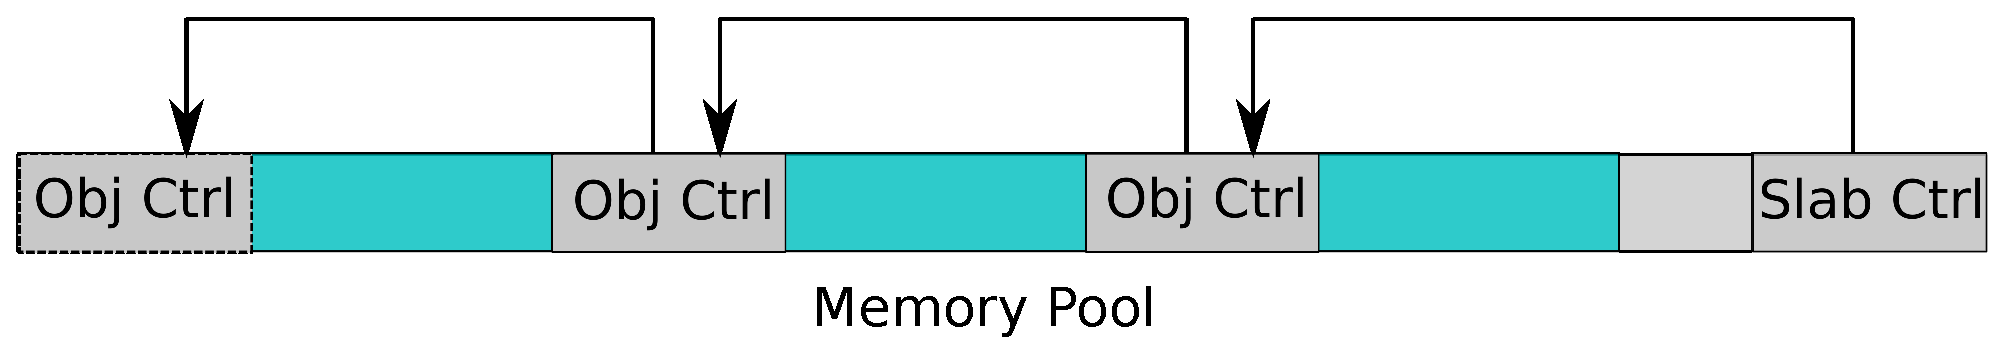
\includegraphics[width=.9\linewidth]{slab-small}

\end{frame}

\begin{frame}
\frametitle{SLAB Allocator}
\framesubtitle{Организация SLAB-а больших объектов объектов}

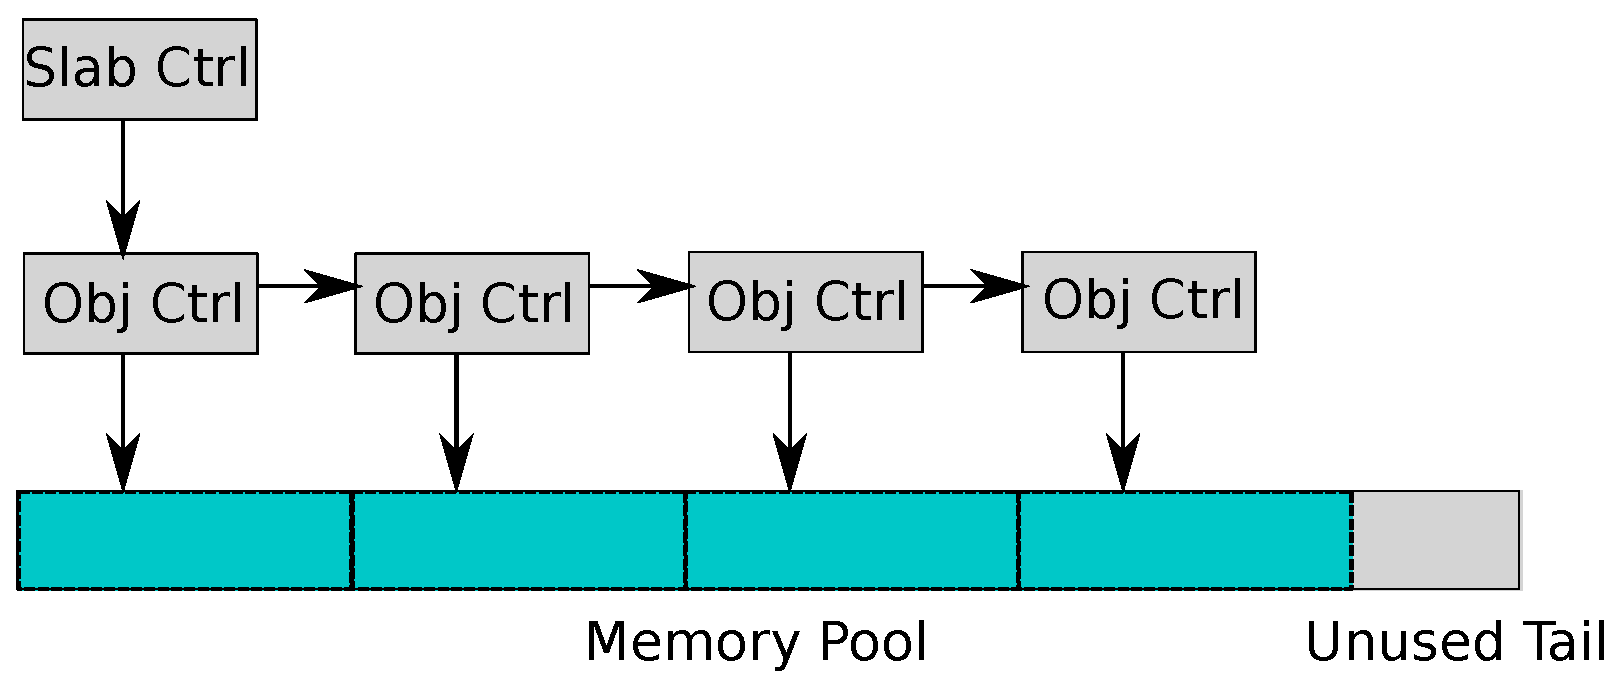
\includegraphics[width=.9\linewidth]{slab-large}

\end{frame}

\begin{frame}
\frametitle{SLAB Allocator}
\framesubtitle{Детали реализации}

\begin{itemize}
  \item Для SLAB-ов больших объектов управляющие структуры нужно аллоцировать отдельно - используя SLAB-ы маленьких объектов.
  \item При освобождении объекта нам нужно найти SLAB из которого он аллоцирован, это можно делать используя словарь (dict, map) или (гораздо проще) используя дескриптор PAGE.
  \item Для SLAB-ов больших объектов ObjCtrl необходим только когда объект свободен, когда объект объект был аллоцирован ObjCtrl больше не нужен.
\end{itemize}
\end{frame}

\begin{frame}
\frametitle{SLAB Allocator}
\framesubtitle{malloc/free}

Используя Buddy Allocator и Slab Allocator можно создать аллокатор общего назначения (malloc/free):
\begin{itemize}
  \item Buddy Allocator - для аллокации пулов памяти для SLAB-ов и для аллокации памяти для больших объектов;
  \item набор предварительно созданных SLAB Allocator-ов с разными размерами объектов - для аллокации маленьких объектов;
\end{itemize}
\end{frame}

\begin{frame}
\frametitle{SLAB Allocator}
\framesubtitle{Объекты одного типа}

Мы можем создавать SLAB Allocator-ы под специфичные нужды и не использовать аллокатор общего назначения:
\begin{itemize}
  \item можно повысить надежность - уменьшив вероятность, что кто-то, по ошибке, испортит нашу память, или, наоборот, что мы испортим чужую;
  \item меньше конкуренция за ресурсы - аллокатором общего назначения пользуются все, а специальным аллокатором только мы;
  \item можно сэкономить на инициализации (далее подробнее);
\end{itemize}
\end{frame}

\begin{frame}
\frametitle{SLAB Allocator}
\framesubtitle{Объекты одного типа}

Многие поля объекта естественным образом оказываются в "инициализированном" состоянии при освобождении объекта:

\begin{itemize}
  \item если объект хранит mutex или spinlock (или какой-то другой примитив синхронизации), то перед освобождением он должен быть отпущен;
  \item если объект хранит счетчик ссылок, то перед освобождением он, зачастую, равен нулю;
  \item если объект хранит список или корень дерева, то перед освобождением они, зачастую, будут пустыми;
\end{itemize}

Такие поля достаточно инициализировать один раз -- экономия на инициализации.

\end{frame}

\begin{frame}
\frametitle{SLAB Allocator}
\framesubtitle{Cache Coloring}

Иногда, при использовании SLAB Allocator-а для достаточно больших объектов, в пуле памяти могут быть неиспользуемые "хвосты" - размер пула не делится нацело на размер объекта.

Этим неиспользуемым хвостам можно найти полезное применение - Cache Coloring.

\end{frame}

\begin{frame}
\frametitle{SLAB Allocator}
\framesubtitle{Cache Coloring}

\begin{columns}[T]

  \begin{column}{.3\textwidth}
    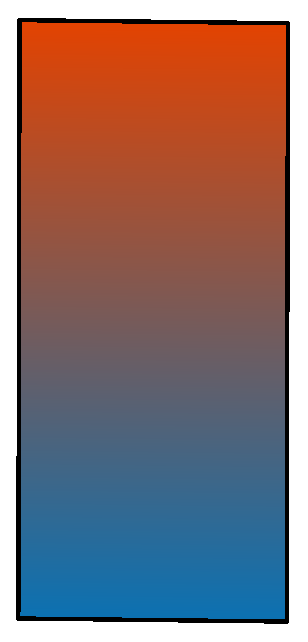
\includegraphics[width=.8\linewidth]{obj-hotmap}
  \end{column}

  \begin{column}{.7\textwidth}
    \begin{itemize}
      \item "горячие" поля, обычно, в начале:
        \begin{itemize}
          \item указатели (следующий/предыдущий, левый/правый)
          \item ключи для поиска (обычно короткие)
          \item флаги и примитивы синхронизации
        \end{itemize}
      \item "холодные" поля, обычно, в конце:
        \begin{itemize}
          \item значения, которые мы ищем (могут быть большими)
        \end{itemize}
    \end{itemize}
  \end{column}

\end{columns}

\end{frame}

\begin{frame}
\frametitle{SLAB Allocator}
\framesubtitle{Cache Coloring}

\begin{columns}[T]

  \begin{column}{.3\textwidth}
    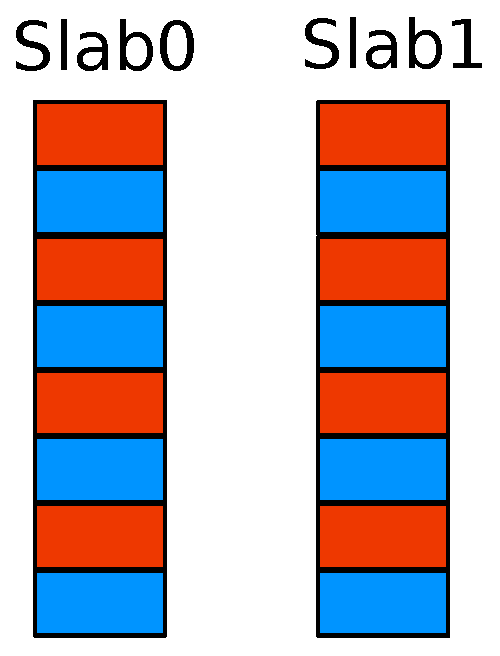
\includegraphics[width=\linewidth]{slab-color0}
  \end{column}

  \begin{column}{.7\textwidth}
    \begin{itemize}
      \item "горячие" поля объектов в Slab0 конкурируют с "горячими" полями объектов в Slab1 за место в процессорном кеше
      \item "холодные" поля конкурируют с "холодными" полями
      \item "холодные" поля используются редко - растрата кеша, лучше поделить его между "горячими" полями
    \end{itemize}
  \end{column}

\end{columns}

\end{frame}

\begin{frame}
\frametitle{SLAB Allocator}
\framesubtitle{Cache Coloring}

\begin{columns}[T]

  \begin{column}{.3\textwidth}
    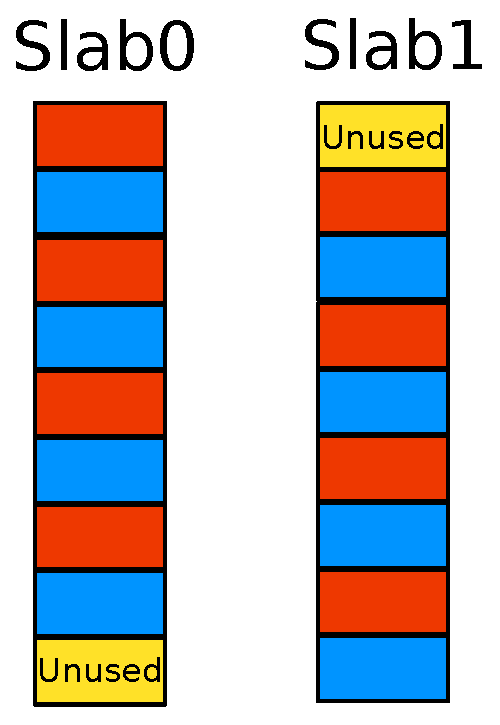
\includegraphics[width=\linewidth]{slab-color1}
  \end{column}

  \begin{column}{.7\textwidth}
    \begin{itemize}
      \item "горячие" поля объектов в Slab0 и Slab1 занимают весь кеш
      \item "холодные" поля поднимаются в кеш, только когда они нужны
    \end{itemize}
  \end{column}

\end{columns}

\end{frame}


  \begin{frame}
\frametitle{Ссылки}

\begin{itemize}
  \item The Art of Computer Programming. Volume 1, 2.5. Donald Knuth - обзор простых алгоритмов аллокации и их поведения;
  \item The Slab Allocator: An Object-Caching Kernel Memory Allocator. Jeff Bonwick - описание классического SLAB Allocator-а;
  \item Magazines and Vmem: Extending the Slab Allocator to Many CPUs and Arbitraray Resources. Jeff Bonwick, Jonathan Adams - продолжение истории SLAB Allocator-а;
  \item Slab allocators in the Linux Kernel: SLAB, SLOB, SLUB. Christoph Lameter - о реализации кеширующих аллокаторов в ядре Linux.
\end{itemize}
\end{frame}


%  \begin{frame}
%    \bibliography{lec1}{}
%    \bibliographystyle{apalike}
%  \end{frame}

\end{document}
